%\documentclass[12pt]{article}  % standard LaTeX, 12 point type
\documentclass[sigconf]{acmart}

\usepackage{booktabs} % For formal tables
\usepackage{multirow}
\usepackage{listings}   

\usepackage{amsfonts,latexsym}
\usepackage{amsthm}
\usepackage{amssymb}
\usepackage[utf8x]{inputenc} % Кодировка
\usepackage[english]{babel} % Многоязычность
\usepackage{amsmath}
\usepackage{tikz}
\usetikzlibrary{automata,positioning}
\usetikzlibrary{graphs, graphs.standard, quotes}
\usetikzlibrary{arrows,decorations.pathmorphing,backgrounds,positioning,fit,petri}


\usepackage{algpseudocode}
\usepackage{algorithm}
\usepackage{caption}
\usepackage{algorithmicx}
\usepackage{systeme}



\newtheorem{theorem}{Theorem}[section]
\newtheorem{proposition}[theorem]{Proposition}
\newtheorem{lemma}[theorem]{Lemma}
\newtheorem{corollary}[theorem]{Corollary}
\newtheorem{conjecture}[theorem]{Conjecture}

\theoremstyle{definition}
\newtheorem{definition}{Определение}[section]
\newtheorem{example}{Example}[section]

% unnumbered environments:

\theoremstyle{remark}
\newtheorem*{remark}{Remark}
\newtheorem*{notation}{Notation}
\newtheorem*{note}{Note}

\setlength{\parskip}{5pt plus 2pt minus 1pt}
%\setlength{\parindent}{0pt}

\usepackage{color}
\usepackage{listings}
\usepackage{caption}
\usepackage{graphicx}
\usepackage{ucs}

\setcounter{MaxMatrixCols}{20}


\newcommand{\tab}[1][0.3cm]{\ensuremath{\hspace*{#1}}}
% A generalized view on parsing and translation
% http://dl.acm.org/citation.cfm?id=2206331
\title{Rytter-style Algorithm for Context-Fre Path Querying}

\author{Semyon Grigorev}
\orcid{0000-0002-7966-0698}
\affiliation{%
  \institution{Saint Petersburg State University}
  \streetaddress{7/9 Universitetskaya nab.}
  \city{St. Petersburg}
  \country{Russia}
  \postcode{199034}
}
\email{semen.grigorev@jetbrains.com}


\author{Ekaterina Shemetova}
\affiliation{%
  \institution{Saint Petersburg State University}
  \streetaddress{7/9 Universitetskaya nab.}
  \city{St. Petersburg}
  \country{Russia}
  \postcode{199034}
}
\email{katyacyfra@gmail.com}




\date{\today}

\textwidth=190mm
\textheight=250mm
\topmargin=-20mm
\oddsidemargin=-15mm
\evensidemargin=-15mm


\begin{document}

\algtext*{EndWhile}% Remove "end while" text
\algtext*{EndIf}% Remove "end if" text
\algtext*{EndFor}% Remove "end for" text
\algtext*{EndFunction}% Remove "end function" text


%\begin{abstract}
%Abstract
%\end{abstract}

%
% The code below should be generated by the tool at
% http://dl.acm.org/ccs.cfm
% Please copy and paste the code instead of the example below.
%
%\begin{CCSXML}
%<ccs2012>
%<concept>
%<concept_id>10002951.10002952.10002953.10010146</concept_id>
%<concept_desc>Information systems~Graph-based database models</concept_desc>
%<concept_significance>500</concept_significance>
%</concept>
%<concept>
%<concept_id>10002951.10002952.10003197.10010825</concept_id>
%<concept_desc>Information systems~Query languages for non-relational engines</concept_desc>
%<concept_significance>500</concept_significance>
%</concept>
%<concept>
%<concept_id>10011007.10011006.10011008.10011009.10011012</concept_id>
%<concept_desc>Software and its engineering~Functional languages</concept_desc>
%<concept_significance>300</concept_significance>
%</concept>
%<concept>
%<concept_id>10003752.10003766.10003771</concept_id>
%<concept_desc>Theory of computation~Grammars and context-free languages</concept_desc>
%<concept_significance>300</concept_significance>
%</concept>
%</ccs2012>
%\end{CCSXML}

%\ccsdesc[500]{Information systems~Graph-based database models}
%\ccsdesc[500]{Information systems~Query languages for non-relational engines}
%\ccsdesc[300]{Software and its engineering~Functional languages}
%\ccsdesc[300]{Theory of computation~Grammars and context-free languages}

%\keywords{Graph Databases, Language-Constrained Path Problem, Context-Free Path Querying, Parser Combinators, Generalized LL, GLL, Neo4J, Scala}


\maketitle

%\chapter*{Введение}                         % Заголовок
\addcontentsline{toc}{chapter}{Введение}    % Добавляем его в оглавление
\textbf{Актуальность работы}

Статический анализ исходного кода является известной техникой  получения знаний о программе без её исполнения ~\cite{StaticCodeAnalysis3,StaticCodeAnalysis2,StaticCodeAnalysis1}. Статический анализ является неотъемлемой частью многих процессов, связанных с разработкой программного обеспечения (ПО), и может использоваться, например, для упрощения работы с кодом с помощью подсветки синтаксиса языка в программах, навигации по коду, реализации контекстных подсказок. Более того, статический анализ используется для обнаружения ошибок на ранних стадиях разработки, до запуска программы, а также для поиска различных семантических ошибок, которые не могут быть определены обычным синтаксическим анализом.  Также, статический анализ используется при решении задач трансформации исходного кода и реинжиниринге~\cite{reengANT}. Однако во многих языках программирования имеются конструкции, которые существенно затрудняют статический анализ. 

Например, широко используются динамические встроенные языки --- приложение, созданное на одном языке, генерирует программу на другом языке и передаёт её на выполнение в соответствующее окружение. Примерами могут служить динамические SQL-запросы к базам данных из приложений на Java, С++, С\#, формирование HTML-страниц в PHP-приложениях~\cite{DSQLISO,JSP,PHPmySQL}. Генерируемый код собирается из строк таким образом, чтобы в момент выполнения результирующая строка представляла собой корректную программу. Примеры использования встроенных языков представлены в листингах~\ref{lst:dsql1},~\ref{lst:JsJava} и~\ref{lst:PhPSqlHtml}. Следует отметить, что одна программа может генерировать код на нескольких языках (см. листинг~\ref{lst:PhPSqlHtml}). При этом возможно получение частей кода из разных источников (например, учитывать текстовый ввод пользователя, что часто используется для задания фильтров при конструировании SQL-запросов). Использование динамически формируемых программ  позволяет избежать дополнительных накладных расходов, присущих таким технологиям, как ORM\footnote{ORM или Object-Relational Mapping --- технология программирования, которая связывает базы данных с концепциями объектно-ориентированных языков программирования~\cite{ORM}.}, и достичь высокой производительности. Благодаря этому использование динамически генерируемых программ получило широкое распространение и применяется до сих пор. Вместе с этим, несмотря на появление новых технологий, динамическая генерация SQL-запросов активно используется и в настоящее время~\cite{DSQLInActiveUse}.

\fvset{frame=lines,framesep=5pt,fontsize=\small}\

\begin{listing}
    \begin{pyglist}[language=sql,numbers=left,numbersep=5pt]

CREATE PROCEDURE [dbo].[MyProc]  @TABLERes   VarChar(30)
AS
    EXECUTE ('INSERT INTO ' + @TABLERes + ' (sText1)' +
             ' SELECT ''Additional condition: '' + sName' +
             ' from #tt where sAction = ''1000000''')
GO
    \end{pyglist}
\caption{Код с использованием динамического SQL}
\label{lst:dsql1}
\end{listing} 
 
\fvset{frame=lines,framesep=5pt}
\begin{listing}
    \begin{pyglist}[language=java,numbers=left,numbersep=5pt]
import javax.script.*;  
public class InvokeScriptFunction {  
    public static void main(String[] args) throws Exception {  
        ScriptEngineManager manager = new ScriptEngineManager();  
        ScriptEngine engine = manager.getEngineByName("JavaScript");  
        // JavaScript code in a String  
        String script = 
            "function hello(name) { print('Hello, ' + name); }";  
        // evaluate script  
        engine.eval(script);  
        // javax.script.Invocable is an optional interface.  
        // Check whether your script engine implements or not!  
        // Note that the JavaScript engine implements
        // Invocable interface.  
        Invocable inv = (Invocable) engine;  
        // invoke the global function named "hello"  
        inv.invokeFunction("hello", "Scripting!!" );  
    }  
}
    \end{pyglist}
\caption{Вызов JavaScript из Java}
\label{lst:JsJava}
\end{listing}


\fvset{frame=lines,framesep=5pt}
\begin{listing}
    \begin{pyglist}[language=php,numbers=left,numbersep=5pt]

<?php
    // Embedded SQL
    $query = 'SELECT * FROM ' . $my_table; 
    $result = mysql_query($query);
    
    // HTML markup generation
    echo "<table>\n";
    while ($line = mysql_fetch_array($result, MYSQL_ASSOC)) {
        echo "\t<tr>\n";    
        foreach ($line as $col_value) {
            echo "\t\t<td>$col_value</td>\n";
        }
        echo "\t</tr>\n";
    }
    echo "</table>\n";
?>
    \end{pyglist}
\caption{Использование нескольких встроенных в PHP языков (MySQL, HTML)}
\label{lst:PhPSqlHtml}
\end{listing}



Динамически формируемые выражения часто конструируются с помощью таких операций, как конкатенация в циклах или условных предложениях, или в рекурсивных процедурах. Это затрудняет статический анализ и приводит к получению множества возможных значений для каждого выражения в момент выполнения. Вследствие этого фрагменты динамически формируемого кода воспринимаются компилятором исходного языка как простые строки, не подлежащие дополнительному анализу, а это, в свою очередь, приводит к высокой вероятности возникновения ошибок во время выполнения программы. В худшем случае такая ошибка не приведёт к прекращению работы приложения, что указало бы на проблемы, однако целостность данных при этом может оказаться нарушена. Более того, использование динамически формируемых выражений затрудняет не только разработку информационных систем, так и также и реинжиниринг, поскольку в последнем случае важно автоматизировать перенос системы на новые зыки и платформы, что невозможно без качественного статического анализа. Например, при наличии в коде приложения динамически формируемых SQL-запросов нельзя точно ответить на вопрос о том, с какими элементами базы данных не взаимодействует система, и удалить их. При переносе такой системы на другую СУБД необходимо гарантировать, что для всех динамически формируемых выражений значение в момент выполнения будет корректным кодом на языке новой СУБД~\cite{JSquash}. Следует отметить, что отсутствие статического анализа динамически формируемых программ не позволяет реализовывать для них стандартную функциональность интегрированных сред разработки (Integrated Development Environment, IDE) --- подсветку синтаксиса и автодополнение, рефакторинг кода и т.д. Такая функциональность значительно упрощает процесс разработки и отладки приложений и полезна не только для основного языка, но и для встроенных языков. 

Для решения всех перечисленных выше задач необходимы инструменты, проводящие статический анализ динамически формируемых программ. Такой анализ может дать существенную информацию о таких программах, поскольку редко встречается ситуация полной динамической неопределённости (например, при создании динамических программ исключительно на основе пользовательского ввода). В большинстве случаев, имея программу, генерирующую динамические вставки, с помощью статического анализа можно получить достаточно информации для решения поставленных выше задач. Решению этой проблемы и посвящена данная диссертационная работа. 


\textbf{Степень разработанности темы}

Существуют классические исследования, посвященные разработке компиляторов --- работы А.~Ахо~\cite{Dragon}, А.~Брукера~\cite{CompilerCompiler}, С.~Джонсона~\cite{yaccBook},  Б.К.Мартыненко~\cite{Martinenko1, Martinenko2}  и др.  Однако содержащиеся там алгоритмы синтаксического анализа не могут быть применены к решению задачи анализа динамически формируемых программ, поскольку предназначены для обработки входных данных, представимых в видн линейной последовательности символов, а такое представление динамически формируемых программ не всегда возможно.

Методы обобщённого синтаксического анализа, лежащие в основе данной работы, изложены в трудах таких учёных как Масару Томита (Masaru Tomita)~\cite{Tomita}, Элизабет Скотт (Elizabeth Scott) и Адриан Джонстон (Adrian Johnstone)~\cite{RNGLR,RIGLR} из университета Royal Holloway (Великобритания), Ян Рекерс (Jan Rekers, University of Amsterdam)~\cite{SPPF}, Элко Виссер (Eelco Visser)~\cite{RNGLRSyntaxerror2,RNGLRSyntaxerror3} и других.

Анализу динамически формируемых строковых выражений посвящены работы таких зарубежных учёных как Кюнг-Гу Дох (Kyung-Goo Doh)~\cite{LrAbstract1,LrAbstract2,LRAbstractParsingSema}, Ясухико Минамиде (Minamide Yasuhiko)~\cite{PHPSA}, Андерс Мёллер (Anders M{\o}ller)~\cite{JSA} и отечественных учёных А.А.~Бреслава~\cite{Alvor1,Alvor2} и других. Хорошо изучены вопросы проверки корректности динамически формируемых выражений и поиска фрагментов кода, уязвимых для SQL-инъекций~\cite{SQLInjection,Dasgupta:2009:SAF:1546683.1547548}. Однако данные работы исследуют отдельные аспекты проблемы статического анализа динамически формируемых программ, оставляя в стороне создание готовых алгоритмов (в частности, не строят структурное представление анализируемых программ). В связи с этим возникают проблемы масштабируемости данных результатов, например, создание на их основе более сложных видов статического анализа.

Так же важным является предоставление компонентов, упрощающих создание новых инструментов для решения конкретных задач. Данных подход хорошо исследован в области разработки компиляторов, где широкое распространение получили генераторы анализаторов и пакеты стандартных библиотек (работы А.~Ахо~\cite{Dragon}, А.~Брукера~\cite{CompilerCompiler}, С.~Джонсона~\cite{yaccBook} и др.). 

В работах отечественных учёных М.Д.~Шапот и Э.В.~Попова~\cite{DynamicDSQLTranslation}, а так же зарубежных учёных Антони Клеви (Anthony Cleve), Жан-Люк Эно (Jean-Luc Hainaut)~\cite{DSQLReverseEngineering}, Йост Виссер (Joost Visser)~\cite{DSQLQualityMesure} и других рассматриваются различные аспекты реинжиниринга информационных систем, использующих встроенные SQL-запросы, однако не формулируется общего метода для решения таких задач. Этот вопрос также не затрагивается в классических работах, посвященных реинжиниригу~\cite{SoftwareReeng1, reengANT, SoftwareReeng2, SoftwareReeng3}. Однако разработка такого метода является актуальной задачей.

Таким образом, актуальной является задача дальнейшего исследования статического анализа динамически формируемых строковых выражений. Кроме этого важным является решение вопросов практического применения средств анализа динамически формируемого кода: упрощение разработки инструментов анализа и создание методов их применения в реинжиниринге программного обеспечения.
\textbf{Объект исследования}

Объектом исследования являются методы, алгоритмы и программные средства обработки динамически формируемых программ, а также задача реинжиниринга информационных систем.

\textbf{Цель и задачи диссертационной работы}

\textbf{Целью} данной работы является создание комплексного подхода к статическому синтаксическому анализу динамически формируемых программ.

Достижение поставленной цели обеспечивается решением следующих \textbf{задач}.
\begin{enumerate}
    \item Разработать универсальный алгоритм синтаксического анализа динамически формируемых программ, не зависящий от целевого языка программирования и допускающий реализацию различных видов статического анализа. 
    \item Создать архитектуру инструментария для автоматизации разработки программных средств статического анализа динамически формируемых программ.
    \item Создать метод реинжиниринга динамически формируемых программ.
\end{enumerate}

\textbf{Методология и методы исследования}

Методология исследования основана на подходе к спецификации и анализу формальных языков, активно развивающемуся с 50-х годов 20-го века (см., например, работы Н. Хомского~\cite{chomskyMethod ,chomskySyntactic}). В последствии этот подход получил широкое распространение в областях, связанных с обработкой языков программирования.
Основными элементами данного подхода являются алфавит и грамматика языка, разбиение автоматической обработки языка на выполнение таких шагов как лексический, синтаксический и семантический анализ. Решаемые в связи с этим задачи связаны с поиском эффективных алгоритмов, выполняющих эти шаги. 

В работе применяется алгоритм обобщённого восходящего синтаксического анализа RNGLR~\cite{RNGLR}, созданный Элизабет Скотт (Elizabeth Scott) и Адриан Джонстон (Adrian Johnstone) из университета Royal Holloway (Великобритания). Для компактного хранения леса вывода использовалась структура данных Shared Packed Parse Forest (SPPF), которую предложил Ян Рекерс (Jan Rekers, University of Amsterdam)~\cite{SPPF}.

Доказательство завершаемости и корректности предложенного алгоритма проводилось с применением теории формальных языков, теории графов и теории сложности алгоритмов. Приближение множества значений динамически формируемого выражения строилось в виде регулярного множества, описываемого с помощью конечного автомата.


\textbf{Положения, выносимые на защиту}
\begin{enumerate}
    \item Разработан алгоритм синтаксического анализа динамически формируемых программ, позволяющий обрабатывать произвольную регулярную аппроксимацию множества значений выражения в точке выполнения, реализующий эффективное управление стеком и гарантирующий конечность представления леса вывода. Доказана завершаемость и корректность предложенного алгоритма при обработке регулярной аппроксимации, представимой в виде произвольного конечного автомата без $\varepsilon$-переходов. 
    \item Создана архитектура инструментария для разработки программных средств статического анализа динамически формируемых программ.
    \item Разработан метод анализа и обработки динамически формируемых программ в проектах по реинжинирингу информационных систем. 
\end{enumerate}

\textbf{Научная новизна работы}

Научная новизна полученных в ходе исследования результатов заключается в следующем.

\begin{enumerate}

\item Алгоритм, предложенный в диссертации, отличается от аналогов (работы Андрея Бреслава~\cite{Alvor1, Alvor2}, Кюнг-Гу Дох~\cite{LrAbstract1, LrAbstract2}, Ясухико Минамиде~\cite{PHPSA}) возможностью построения компактной структуры данных, содержащей деревья вывода для всех корректных значений выражения. Это позволяет использовать результаты работы алгоритма для проведения более сложных видов анализа. Алгоритмы, представленные в (JSA~\cite{JSA}~\cite{Alvor1, Alvor2}, PHPSA~\cite{PHPSA}) предназначены только для проверки корректности выражений, основанной на решении задачи о включении одного языка в другой. Выполнение более сложных видов анализа, трансформаций или построения леса разбора не предполагается. 

\item Новизна представленной архитектуры заключается в том, что она позволяет создать платформу для разработки целевых инструментов, решающих широкий круг задач анализа динамически формируемого кода. Существующие архитектуры готовых инструментов (JSA, PHPSA, Alvor, Varis) предназначены для решения конкретных задач для определённых языков. Решение новых задач или поддержка других языков с помощью этих инструментов затруднены ввиду ограничений, накладываемых архитектурой и возможностями используемого алгоритма анализа. 

\item Метод анализа и обработки встроенного программного кода в проектах по реинжинирингу информационных систем предложен впервые. К.В.~Ахтырченко и Т.П.~Сорокваша отмечают~\cite{SoftwareReengMethods}, что существующие работы в области реинжиниринга программного обеспечения либо содержат высокоуровневые решения, не касающиеся деталей, важных при решении прикладных задач (например, работы К. Вагнера~\cite{SoftwareReeng3}, Х. Миллера~\cite{SoftwareReeng2}), либо являются набором подходов к решению конкретных задач (например, работы~\cite{SoftwareReeng1, reengANT, boulychev}). При этом, встроенный программный код часто не учитывается. С другой стороны, работы М.Д.~Шапот и Э.В.~Попова~\cite{DynamicDSQLTranslation}, С.Л.~Трошина~\cite{reengANT}, А.~Клеви~\cite{DSQLReverseEngineering}  посвящены решению конкретных задач обработки встроенного программного кода в контексте реинжиниринга информационных систем, но не предлагают обобщённого и масштабируемого метода.

\end{enumerate}


\textbf{Теоретическая и практическая значимость работы}

Теоретическая значимость диссертационного исследования заключается в разработке формального алгоритма синтаксического анализа динамически формируемого кода, решающего задачу построения конечного представления леса вывода, не решенную полностью ранее, а также в формальном доказательстве завершаемости и корректности разработанного алгоритма. 

На основе полученных в работе научных результатов был разработан инструментарий (Software Development Kit, SDK), предназначенный для создания средств статического анализа динамически формируемых программ. 
С использованием разработанного инструментария было реализовано расширение к инструменту ReSharper (ООО ``ИнтеллиДжей Лабс'', Россия), предоставляющее поддержку встроенного T-SQL в проектах на языке программирования C\# в среде разработки Microsoft Visual Studio. Так же было выполнено внедрение результатов работы в промышленный проект по переносу хранимого SQL-кода с MS-SQL Server 2005 на Oraclе 11gR2 (ЗАО ``Ланит-Терком'', Россия). 

\textbf{Степень достоверности и апробация результатов}

Достоверность и обоснованность результатов исследования опирается на использование формальных методов исследуемой области, проведенные доказательства, рассуждения и эксперименты.

Основные результаты работы были доложены на ряде научных конференций: SECR-2012, SECR-2013, SECR-2014, TMPA-2014, Parsing@SLE-2013, Рабочий семинар ``Наукоемкое программное обеспечение'' при конференции PSI-2014. Доклад на SECR-2014 награждён премией Бертрана Мейера за лучшую исследовательскую работу в области программной инженерии. Дополнительной апробацией является то, что разработка инструментальных средств на основе предложенного алгоритма была поддержана Фондом содействия развитию малых форм предприятий в технической сфере (программа УМНИК~\cite{UMNIC}, проекты \textnumero~162ГУ1/2013 и \textnumero~5609ГУ1/2014).

\textbf{Публикации по теме диссертации}

Все результаты диссертации изложены в 7 научных работах, из которых 3~\cite{YCArticle,SELforIDEru,AbstractGLL}, содержащие основные результаты, опубликованы в журналах из ‘’Перечня российских рецензируемых научных журналов, в которых должны быть опубликованы основные научные результаты диссертаций на соискание ученых степеней доктора и кандидата наук’’, рекомендовано ВАК. 
1 работа~\cite{GLRAbsPars} индексируются Scopus. В работах, написанных в соавторстве, вклад автора определяется следующим образом.  В~\cite{Syrcose} С. Григорьеву принадлежит реализация ядра платформы YaccConstructor. В~\cite{SELforIDEru, AbstractGLL} и~\cite{SELforIDE} С. Григорьеву принадлежит постановка задачи, формулирование требований к разрабатываемым инструментальным средствам, работа над текстом. 
В~\cite{GLRAbsPars} автору принадлежит идея, описание и реализация анализа встроенных языков на основе RNGLR алгоритма.  В~\cite{YCArticle} С. Григорьеву принадлежит реализация инструментальных средств, проведение экспериментов, работа над текстом. В работе~\cite{RelaxedARNGLR} автору принадлежит алгоритм синтаксического анализа динамически формируемого кода.


\textbf{Структура работы}

Диссертация состоит из введения, шести глав, заключения и построена следующим образом. В первой главе приводится обзор области исследования. Рассматриваются подходы к анализу динамически формируемых строковых выражений и соответствующие инструменты. Описывается алгоритм обобщённого восходящего синтаксического анализа RNGLR, взятый за основу в диссертационной работе. Также описываются проекты YaccConstructor и ReSharper SDK, использованные для реализации предложенного в работе инструментария. Во второй главе формализуется основная задача исследования и излагается решающий её алгоритм синтаксического анализа регулярных множеств. Приводится доказательство завершаемости и корректности представленного алгоритма, приводятся примеры. В третьей главе описывается инструментальный пакет YC.SEL.SDK, разработанного на основе алгоритма, описанного во второй главе и предназначеного для разработки инструментов анализа динамически формируемых программ. Описывается архитектура компонентов и особенности их реализации. Также описывается YC.SEL.SDK.ReSharper --- ``обёртка'' для YC.SEL.SDK, позволяющая создавать расширения к ReSharper для поддержки встроенных языков. В четвёртой главе описывается метод реинжиниринга встроенного программного кода.  В пятой главе приводятся результаты экспериментального исследования разработанного алгоритма и инструмента YC.SEL.SDK. Шестая глава содержит результаты сравнения и соотнесения полученных результатов с  существующими аналогами.

\textbf{Благодарности}

А.Н.Терехову, работкникам и администрации компании ЗАО ``Ланит-Терком'' за создания условий для изучения данной темы (организация проектов по реинжинирингу). Я.А.Кириленко за погружение в тему исследования и руководство на начальных этапах. Д.Ю.Булычеву за помощь в уточнении постановки задачи исследования и в написании статей. Студентам и аспирантам кафедры системного программирования Дмитрию Авдюхину, Анастасии Рагозиной, Екатерине Вербицкой, Марине Полубеловой, Иванову Андрею за помощь в реализации предложенных идей и проведение экспериментов. Отдельную благодарность  хочется выразить компании ООО ``ИнтеллиДжей Лабс'' и Андрею Иванову за поддержку исследований. Также хочется поблагодарить А.К.Петренко и В.М.Ицыксона, а также сотрудников ИСП РАН за ценные вопросы и комментарии к работе, позволившие уточнить ряд формулировок и улучшить изложение результатов. 


%\section{Strongly Connected Components Handling}

Steps:
\begin{enumerate}
\item Convert input graph to graph for 2-Dyck querying.
\item Convert graph to one strongly connected component by adding edges with new unique label from 
synks to sources.
\item Convert 2-Dyck grammar to grammar which can accept arbitrary path with 2-Dyck subpaths.
\item Execute modified Rytter for one arbitrary selected vertex and its output edge.
\end{enumerate}

In strongly connected components each vetex is reachcbel from another, but not each path should match 
required constraints.
The idea is to extend grammar by the such way, that it accepts arbitrary path and provide information 
about parts which satisfie to original constraints.
As far as we can reduce any CFPQ to 2-Dyck query, we can fix grammar as follows.
\begin{align*}
S & \rightarrow A \ S_1 \ | \ C \ S_2  \ | \ S \ S \ | \ A \ B \ | \ C \ D
\\
S_1 & \rightarrow S \ B 
\\
S_2 & \rightarrow S \ D 
\\
A & \rightarrow a 
\\
B & \rightarrow b 
\\
C & \rightarrow c 
\\
D & \rightarrow d
\end{align*}

Let label of new edges which added in order to convert graph to single SCC is $E$.
Arbitrary path consists of 2-Dyck subpaths connected by unbalanced parts.
We can specify grammar for these paths.

\begin{align*}
S'  \rightarrow & a \ | \ b \ | \ c \ | \ d \ |  \ e \ |
\\
  & \ A \ S' \ | \ B \ S' \ | \ C \ S' \ | \ D \ S' \ | \ E \ S' \ | \ S' \ S' \ |  
 \\
  & \ A \ S_1 \ | \ C \ S_2 \ | \ S \ S \ | \ A \ B \ | \ C \ D \   
\\
S   \rightarrow & A \ S_1 \ | \ C \ S_2  \ | \ S \ S \ | \ A \ B \ | \ C \ D
\\
S_1  \rightarrow & S \ B 
\\
S_2  \rightarrow & S \ D 
\\
A  \rightarrow & a 
\\
B  \rightarrow & b 
\\
C  \rightarrow & c 
\\
D  \rightarrow & d
\\
E  \rightarrow & e
\end{align*}

Now we can start processing from one arbitrary selected vertex.

Scheme of proof.
\begin{enumerate}
\item Convertion to 2-Dyck path querying. Look at ection !!!. 
\item Convertion to single SCC. In worst case we should add $|V|$ outgoing edges for each vertes. 
So, time complexity is $O(|V|^2)$.
\item Why can we select arbitrary edge for start?
We can select arbitrarry vertex just because we handle SCC, so all other vertices should be reachcble from selected one.
We should choose outgoing edge from selected vertex in order to fix source vertex in Rytter graph.
\item Rytter
\end{enumerate}
\section{The reduction}

Suppose we have $\Phi$ --- an instance of 3-SAT problem contains $m$ clauses over $k$ variables.

First of all, we should to constract a graph. 
To do it we follow the next steps.
\begin{enumerate}
	\item 
	Let $\gamma_i = \{v_1 \leftarrow b_1, v_2 \leftarrow b_2, \cdots, v_k \leftarrow b_k\}$ where $b_k \in \{0,1\}$.
	For each substitution $\gamma_i$ a vertex $V_{\gamma_i}$ should be created.
	\item For each $V_{\gamma_i}$ the following edges should be added: $\{ (V_{\gamma_i}, [v_j \leftarrow b_l]^+ ,V_{\gamma_i}) \mid v_j \leftarrow b_l \in \gamma_i \}$.
	\item For each clause $(l_1 \vee l_2 \vee l_3)$ the following subgraph should be created.
	First, two new vertices are edded: $c_1$ and $c_2$.
	After that, the following edges for each $l_p$ and for each $\gamma_i$ should be added $$\{(c_1, [v_j \leftarrow b_l]^- ,c_2) \mid b_l = \systeme*{1 \text{ if } l_p = v_j, 0  \text{ if } l_p = \neg v_j} \}.$$
	\item Subgraph for all clauses should be connected sequencially. 
	Suppose we have seqence of subgraps with vertices $$\{(c_1^1,c_2^1),(c_1^2,c_2^2),\cdots,(c_1^m,c_2^m)\}.$$ To connect them we should merge vertices $c_2^{i}$ and $c_1^{i+1}$ for all $i$ except $i=m$.
	After that we fix $c_1^1$ as a start vertex of formula subgraph, and $c_2^m$ as a final vertex of formula subgraph.
    \item Finally, for all $V_{\gamma_i}$ we should add the following edge
    $$
    (V_{\gamma_i}, q ,c_1^1)
    $$
\end{enumerate}

The second part is a query.
Suppose, we have p different substitutions.
The gramamr is following
\begin{align*}
S & \to q \\
S & \to [v_1 \leftarrow b_1]^+ \ S \ [v_1 \leftarrow b_1]^-  \\
  & \mid \cdots \\
  & \mid  [v_k \leftarrow b_k]^+ \ S \ [v_k \leftarrow b_k]^- \\ 
\end{align*}

After that we should applay transformation which is described in the section~\ref{sec:cfpq_to_dyck}. 
As a result we get h-Dyck reachability problem (yes, we can reduce it to 2-Dyck reachability).

\subsection{An Example of Reduction}

Suppose we have the following instance of 3-SAT problem. 
$$
\Phi = (\neg x_1 \vee x_2 \vee \neg x_3) \wedge (\neg x_2 \vee x_1 \vee x_3) \wedge (x_1 \vee \neg x_3 \vee x_2)
$$

Substitutions:
\begin{align*}
\gamma_1 = \{x_1 \leftarrow 0, x_2 \leftarrow 0, x_3 \leftarrow 0\} \\
\gamma_2 = \{x_1 \leftarrow 1, x_2 \leftarrow 0, x_3 \leftarrow 0\} \\
\gamma_3 = \{x_1 \leftarrow 0, x_2 \leftarrow 1, x_3 \leftarrow 0\} \\
\gamma_4 = \{x_1 \leftarrow 0, x_2 \leftarrow 0, x_3 \leftarrow 1\} \\
\gamma_5 = \{x_1 \leftarrow 1, x_2 \leftarrow 1, x_3 \leftarrow 0\} \\
\gamma_6 = \{x_1 \leftarrow 1, x_2 \leftarrow 0, x_3 \leftarrow 1\} \\
\gamma_7 = \{x_1 \leftarrow 0, x_2 \leftarrow 1, x_3 \leftarrow 1\} \\
\gamma_8 = \{x_1 \leftarrow 1, x_2 \leftarrow 1, x_3 \leftarrow 1\} 
\end{align*}

Graph for $\Phi$ is presented in figure~\ref{fig:sat_to_cfpq_graph_example}.

The grammar:
\begin{align*}
S & \to  [x_1 \leftarrow 0]^+ \ S \ [x_1 \leftarrow 0]^- \\
  & \mid [x_2 \leftarrow 0]^+ \ S \ [x_2 \leftarrow 0]^- \\ 
  & \mid [x_3 \leftarrow 0]^+ \ S \ [x_3 \leftarrow 0]^- \\
  & \mid [x_1 \leftarrow 1]^+ \ S \ [x_1 \leftarrow 1]^- \\ 
  & \mid [x_2 \leftarrow 1]^+ \ S \ [x_2 \leftarrow 1]^- \\ 
  & \mid [x_3 \leftarrow 1]^+ \ S \ [x_3 \leftarrow 1]^- \\
  & \mid q \\
\end{align*}

The intuition of such path finding is that substitution vertex ($V_{\gamma_i}$) should provide appropriate values for respective variable in appropriate order to satisfy the given formula.
It can be done by appropriate traversing of loops. 
After that, each edge from $c_i^j$ to  $c_l^k$ ``uses'' provided values to satisfie respective closure, and it can be done if and only if the respective vertex provides value required.
This fact is expressed by usung balanced-bracket grammar.
So, if there exists a path from $V_{\gamma_i}$ to $c_2^3$, such that the corresponded word is derivable from $S$, then $V_{\gamma_i}$ satisfy the given formula. 


\begin{figure*}
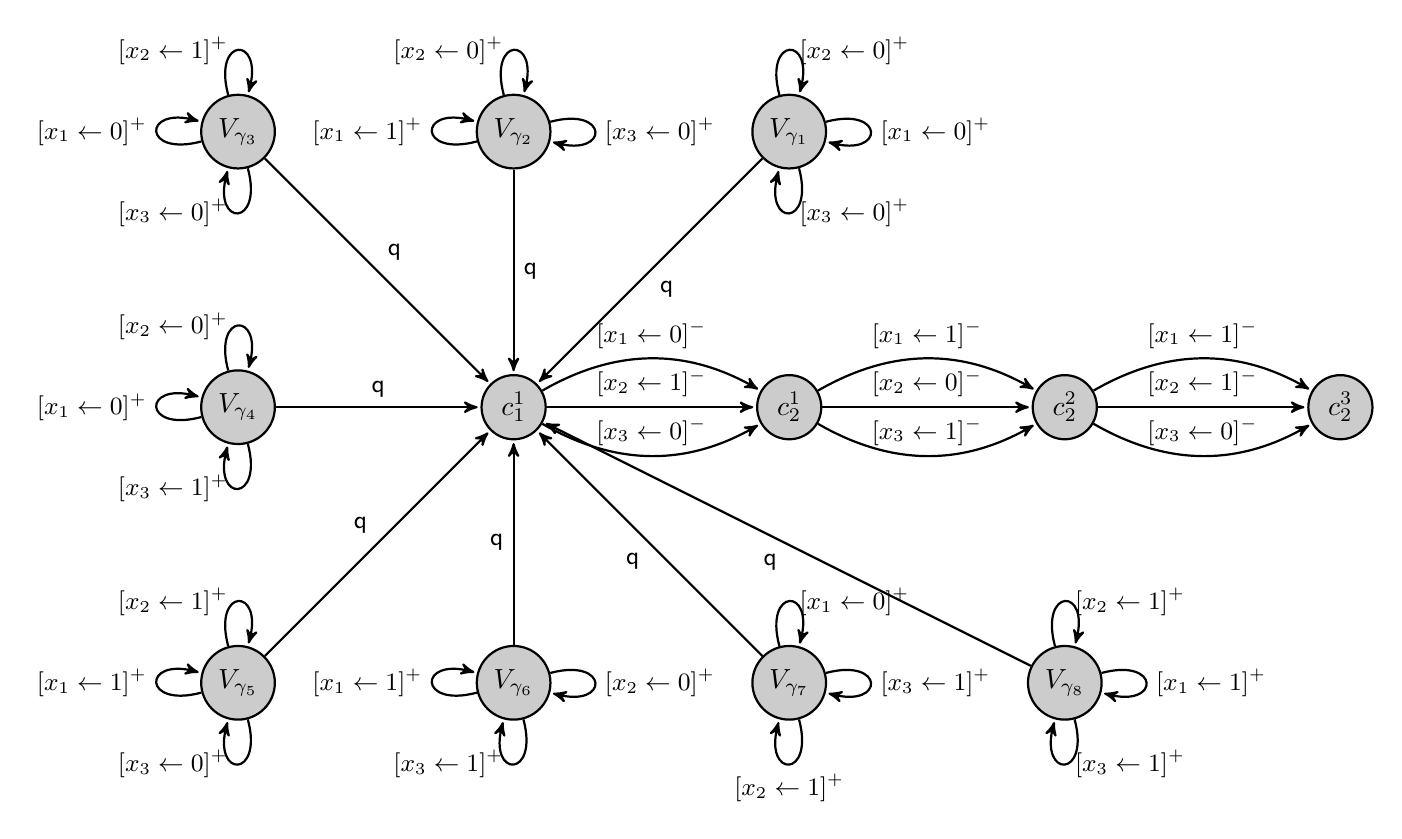
\begin{tikzpicture}[-,>=stealth',shorten >=1pt,auto,node distance=3.5cm,
  thick,main node/.style={circle,fill=black!20,draw}]

  
  \node[main node] (7) [] {$V_{\gamma_3}$};
  \node[main node] (8) [below of=7] {$V_{\gamma_4}$};
  \node[main node] (9) [below of=8] {$V_{\gamma_5}$};


  \node[main node] (1) [right of=8] {$c_1^1$};
  \node[main node] (2) [right of=1] {$c_2^1$};
  \node[main node] (3) [right of=2] {$c_2^2$};
  \node[main node] (4) [right of=3] {$c_2^3$};

  \node[main node] (5) [above of=2] {$V_{\gamma_1}$};
  \node[main node] (6) [above of=1] {$V_{\gamma_2}$};
  \node[main node] (10) [below of=1] {$V_{\gamma_6}$};
  \node[main node] (11) [below of=2] {$V_{\gamma_7}$};
  \node[main node] (12) [below of=3] {$V_{\gamma_8}$};


  \path[-> , every node/.style={font=\sffamily\small}]
    (5) edge [loop right, right] node  {$[x_1 \leftarrow 0]^+$}   (5)    
    (5) edge [loop above, right] node  {$[x_2 \leftarrow 0]^+$}  (5)    
    (5) edge [loop below, right] node  {$[x_3 \leftarrow 0]^+$}  (5)

    (5) edge [] node  {q}  (1)    
    

    (6) edge [loop left, left] node   {$[x_1 \leftarrow 1]^+$}   (6)    
    (6) edge [loop above, left] node  {$[x_2 \leftarrow 0]^+$}  (6)    
    (6) edge [loop right, right] node  {$[x_3 \leftarrow 0]^+$}  (6)

    (6) edge [] node  {q}  (1)    
         


    (7) edge [loop left, left] node   {$[x_1 \leftarrow 0]^+$}   (7)    
    (7) edge [loop above, left] node  {$[x_2 \leftarrow 1]^+$}  (7)    
    (7) edge [loop below, left] node  {$[x_3 \leftarrow 0]^+$}  (7)

    (7) edge [] node   {q}  (1)    
    


    (8) edge [loop left, left] node   {$[x_1 \leftarrow 0]^+$}   (8)    
    (8) edge [loop above, left] node  {$[x_2 \leftarrow 0]^+$}  (8)    
    (8) edge [loop below, left] node  {$[x_3 \leftarrow 1]^+$}  (8)

    (8) edge [] node  {q}  (1)    
    

    (9) edge [loop left, left] node   {$[x_1 \leftarrow 1]^+$}   (9)    
    (9) edge [loop above, left] node  {$[x_2 \leftarrow 1]^+$}  (9)    
    (9) edge [loop below, left] node  {$[x_3 \leftarrow 0]^+$}  (9)

    (9) edge [] node  {q}  (1)    

    
    (10) edge [loop left, left] node   {$[x_1 \leftarrow 1]^+$}   (10)    
    (10) edge [loop right, right] node  {$[x_2 \leftarrow 0]^+$}  (10)    
    (10) edge [loop below, left] node  {$[x_3 \leftarrow 1]^+$}  (10)

    (10) edge [] node   {q}  (1)    

    
    (11) edge [loop above, right] node    {$[x_1 \leftarrow 0]^+$}   (11)    
    (11) edge [loop below, below] node  {$[x_2 \leftarrow 1]^+$}  (11)    
    (11) edge [loop right, right] node  {$[x_3 \leftarrow 1]^+$}  (11)

    (11) edge [] node  {q}  (1)


    (12) edge [loop right, right] node  {$[x_1 \leftarrow 1]^+$}   (12)    
    (12) edge [loop above, right] node  {$[x_2 \leftarrow 1]^+$}  (12)    
    (12) edge [loop below, right] node  {$[x_3 \leftarrow 1]^+$}  (12)

    (12) edge [] node  {q}  (1)    
 

    (1) edge [bend left=30, above] node   {$[x_1 \leftarrow 0]^-$}  (2)
    (1) edge [bend left=0, above] node   {$[x_2 \leftarrow 1]^-$}  (2)
    (1) edge [bend right=30, above] node   {$[x_3 \leftarrow 0]^-$}  (2)
      

    (2) edge [bend left=30, above] node  {$[x_1 \leftarrow 1]^-$}  (3)
    (2) edge [bend left=0, above] node  {$[x_2 \leftarrow 0]^-$}  (3)
    (2) edge [bend right=30, above] node  {$[x_3 \leftarrow 1]^-$}  (3)
   

    (3) edge [bend left=30, above] node  {$[x_1 \leftarrow 1]^-$}  (4)
    (3) edge [bend left=0, above] node  {$[x_2 \leftarrow 1]^-$}  (4)
    (3) edge [bend right=30, above] node  {$[x_3 \leftarrow 0]^-$}  (4)
    
    ;

\end{tikzpicture}
\caption{Example of graph for $\Phi$}
\label{fig:sat_to_cfpq_graph_example}
\end{figure*}

\section{Reduction to $k/3$}

	
Firs step is to split variables into three group of the same size.
Suppose this splitting preserves the order.
So, we have a set of partial substitution. 

By the same way we create vertices for partial subctitutions.


\section{An Example of Reduction $k/3$}

For our example:
\begin{align*}
\gamma_1^1 = \{x_1 \leftarrow 1 \} \\
\gamma_1^2 = \{x_1 \leftarrow 0 \} \\
\gamma_2^1 = \{x_2 \leftarrow 1 \} \\
\gamma_2^2 = \{x_2 \leftarrow 0 \} \\
\gamma_3^1 = \{x_3 \leftarrow 1 \} \\
\gamma_3^2 = \{x_3 \leftarrow 0 \} 
\end{align*}

Grammar:
\begin{align*}
S & \to S_1 \mid S_2 \mid S_3 \mid S_4 \mid S_5 \mid S_6 \mid S_7 \mid S_8\\
S_1 & \to q \mid p^+ \ S_1 \ p^- 
      \mid [x_1 \leftarrow 0]^+ \ S_1 \ [x_1 \leftarrow 0]^- \\ 
    & \mid [x_2 \leftarrow 0]^+ \ S_1 \ [x_2 \leftarrow 0]^- 
      \mid [x_3 \leftarrow 0]^+ \ S_1 \ [x_3 \leftarrow 0]^- \\
S_2 & \to q \\
    & \mid p^+ \ S_2 \ p^- 
      \mid [x_1 \leftarrow 1]^+ \ S_2 \ [x_1 \leftarrow 1]^- \\ 
    & \mid [x_2 \leftarrow 0]^+ \ S_2 \ [x_2 \leftarrow 0]^- 
      \mid [x_3 \leftarrow 0]^+ \ S_2 \ [x_3 \leftarrow 0]^- \\
S_3 & \to q \mid p^+ \ S_3 \ p^- 
      \mid [x_1 \leftarrow 0]^+ \ S_3 \ [x_1 \leftarrow 0]^- \\ 
    & \mid [x_2 \leftarrow 1]^+ \ S_3 \ [x_2 \leftarrow 1]^- 
      \mid [x_3 \leftarrow 0]^+ \ S_3 \ [x_3 \leftarrow 0]^- \\
S_4 & \to q \mid p^+ \ S_4 \ p^- 
      \mid [x_1 \leftarrow 0]^+ \ S_4 \ [x_1 \leftarrow 0]^- \\ 
    & \mid [x_2 \leftarrow 0]^+ \ S_4 \ [x_2 \leftarrow 0]^- 
      \mid [x_3 \leftarrow 1]^+ \ S_4 \ [x_3 \leftarrow 1]^- \\
S_5 & \to q \mid p^+ \ S_5 \ p^- 
      \mid [x_1 \leftarrow 1]^+ \ S_5 \ [x_1 \leftarrow 1]^- \\ 
    & \mid [x_2 \leftarrow 1]^+ \ S_5 \ [x_2 \leftarrow 1]^- 
      \mid [x_3 \leftarrow 0]^+ \ S_5 \ [x_3 \leftarrow 0]^- \\
S_6 & \to q \mid p^+ \ S_6 \ p^- 
      \mid [x_1 \leftarrow 1]^+ \ S_6 \ [x_1 \leftarrow 1]^- \\ 
    & \mid [x_2 \leftarrow 0]^+ \ S_6 \ [x_2 \leftarrow 0]^- 
      \mid [x_3 \leftarrow 1]^+ \ S_6 \ [x_3 \leftarrow 1]^- \\
S_3 & \to q \mid p^+ \ S_7 \ p^- 
      \mid [x_1 \leftarrow 0]^+ \ S_7 \ [x_1 \leftarrow 0]^- \\ 
    & \mid [x_2 \leftarrow 1]^+ \ S_7 \ [x_2 \leftarrow 1]^- 
      \mid [x_3 \leftarrow 1]^+ \ S_7 \ [x_3 \leftarrow 1]^- \\
S_8 & \to q \mid p^+ \ S_8 \ p^- 
      \mid [x_1 \leftarrow 1]^+ \ S_8 \ [x_1 \leftarrow 1]^- \\ 
    & \mid [x_2 \leftarrow 1]^+ \ S_8 \ [x_2 \leftarrow 1]^- 
      \mid [x_3 \leftarrow 1]^+ \ S_8 \ [x_3 \leftarrow 1]^- \\
\end{align*}

\begin{figure*}
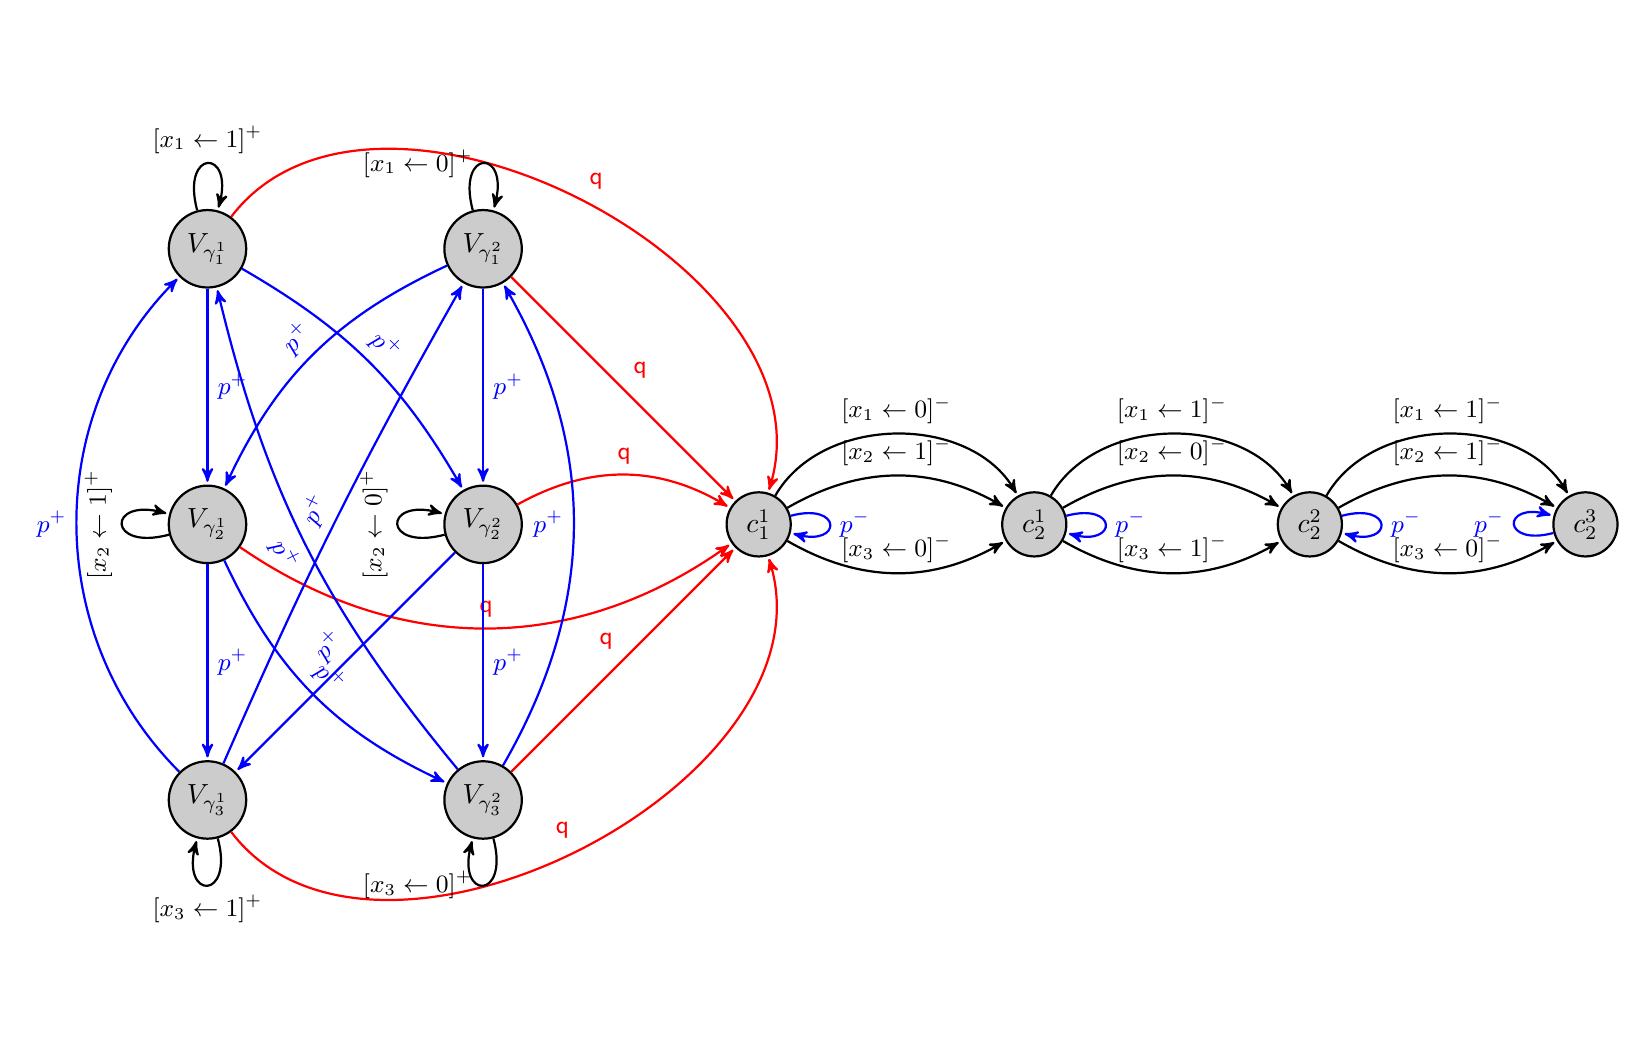
\begin{tikzpicture}[-,>=stealth',shorten >=1pt,auto,node distance=3.5cm,
  thick,main node/.style={circle,fill=black!20,draw}]

  
  \node[main node] (6) [] {$V_{\gamma_1^1}$};
  \node[main node] (7) [right of =6] {$V_{\gamma_1^2}$};
  \node[main node] (8) [below of=6] {$V_{\gamma_2^1}$};
  \node[main node] (9) [right of=8] {$V_{\gamma_2^2}$};
  \node[main node] (10) [below of=8] {$V_{\gamma_3^1}$};
  \node[main node] (11) [right of=10] {$V_{\gamma_3^2}$};
  


  \node[main node] (1) [right of=9] {$c_1^1$};
  \node[main node] (2) [right of=1] {$c_2^1$};
  \node[main node] (3) [right of=2] {$c_2^2$};
  \node[main node] (4) [right of=3] {$c_2^3$};

  
  \path[-> , every node/.style={font=\sffamily\small}]
    (6) edge [loop above, above] node  {$[x_1 \leftarrow 1]^+$}   (6)    
    
    (6) edge [bend left = 80, color=red] node  {q}  (1)        
    (6) edge [color=blue] node  {$p^+$}  (8)
    (6) edge [color=blue, sloped, bend left=15] node  {$p^+$}  (9)                


    (7) edge [loop above, left] node  {$[x_1 \leftarrow 0]^+$}   (7)    
    
    (7) edge [color=red] node {q}  (1)        
    (7) edge [color=blue, sloped, above, bend right=20] node  {$p^+$}  (8)
    (7) edge [color=blue] node  {$p^+$}  (9) 


    (8) edge [loop left, sloped, above] node  {$[x_2 \leftarrow 1]^+$}   (8)    
    
    (8) edge [bend right=35, sloped, above, color=red] node  {q}  (1)        
    (8) edge [color=blue] node  {$p^+$}  (10)
    (8) edge [color=blue, sloped, bend right=20] node  {$p^+$}  (11) 

    (9) edge [loop left, above, sloped] node  {$[x_2 \leftarrow 0]^+$}   (9)    
    
    (9) edge [color=red,bend left] node  {q}  (1)        
    (9) edge [color=blue, sloped, above] node  {$p^+$}  (10)
    (9) edge [color=blue] node  {$p^+$}  (11)     
    
    (10) edge [loop below, below] node  {$[x_3 \leftarrow 1]^+$}   (10)    
    
    (10) edge [bend right=80,color=red] node  {q}  (1)        
    (10) edge [bend left=45, color=blue] node  {$p^+$}  (6)
    (10) edge [bend left=3, color=blue, above, sloped] node  {$p^+$}  (7) 
    
    (11) edge [loop below, left] node  {$[x_3 \leftarrow 0]^+$}   (11)    
    
    (11) edge [color=red] node  {q}  (1) 
    (11) edge [bend left=13, color=blue, below, sloped] node  {$p^+$}  (6)
    (11) edge [bend right, color=blue] node  {$p^+$}  (7)


    (1) edge [bend left=60, above] node  {$[x_1 \leftarrow 0]^-$}  (2)
    (1) edge [bend left=30, above] node  {$[x_2 \leftarrow 1]^-$}  (2)
    (1) edge [bend right=30, above] node  {$[x_3 \leftarrow 0]^-$}  (2)
    (1) edge [loop right, right, color=blue] node {$p^-$} (1)
    


    (2) edge [bend left=60, above] node  {$[x_1 \leftarrow 1]^-$}  (3)
    (2) edge [bend left=30, above] node  {$[x_2 \leftarrow 0]^-$}  (3)
    (2) edge [bend right=30, above] node  {$[x_3 \leftarrow 1]^-$}  (3)
    (2) edge [loop right, right, color=blue] node {$p^-$} (2)
    

    (3) edge [bend left=60, above] node  {$[x_1 \leftarrow 1]^-$}  (4)
    (3) edge [bend left=30, above] node  {$[x_2 \leftarrow 1]^-$}  (4)
    (3) edge [bend right=30, above] node  {$[x_3 \leftarrow 0]^-$}  (4)
    (3) edge [loop right, right, color=blue] node {$p^-$} (3)
    
    (4) edge [loop left, left, color=blue] node {$p^-$} (4)
    

    ;

\end{tikzpicture}
\caption{Example of graph for $\Phi$}
\label{fig:sat_to_cfpq_graph_example}
\end{figure*}


\section{Improved Reduction to $k/3$}

	
Firs step is to split variables into three group of the same size.
Suppose this splitting preserves the order.
So, we have a set of partial substitution. 

By the same way we create vertices for partial subctitutions.


\section{An Example of Improved Reduction $k/3$}

For our example:
\begin{align*}
\gamma_1^1 = \{x_1 \leftarrow 1 \} \\
\gamma_1^2 = \{x_1 \leftarrow 0 \} \\
\gamma_2^1 = \{x_2 \leftarrow 1 \} \\
\gamma_2^2 = \{x_2 \leftarrow 0 \} \\
\gamma_3^1 = \{x_3 \leftarrow 1 \} \\
\gamma_3^2 = \{x_3 \leftarrow 0 \} 
\end{align*}

Grammar:
\begin{align*}
S & \to S_{\gamma_1} \mid S_{\gamma_2} \mid S_{\gamma_3} \mid S_{\gamma_4} \mid S_{\gamma_5} \mid S_{\gamma_6} \mid S_{\gamma_7} \mid S_{\gamma_8}\\
S_1 & \to q  
      \mid [x_1 \leftarrow 1]^+ \ S_1 \ [x_1 \leftarrow 1]^- \\ 
S_2 & \to q  
      \mid [x_1 \leftarrow 0]^+ \ S_2 \ [x_1 \leftarrow 0]^- \\ 
S_3 & \to q  
      \mid [x_2 \leftarrow 1]^+ \ S_3 \ [x_2 \leftarrow 1]^- \\ 
S_4 & \to q 
      \mid [x_2 \leftarrow 0]^+ \ S_4 \ [x_2 \leftarrow 0]^- \\ 
S_5 & \to q
      \mid [x_3 \leftarrow 1]^+ \ S_5 \ [x_3 \leftarrow 1]^- \\ 
S_6 & \to q
      \mid [x_3 \leftarrow 0]^+ \ S_6 \ [x_3 \leftarrow 0]^- \\ 
S_{\gamma_1} & \to S_2 \mid S_4 \mid S_6 \mid S_{\gamma_1} \ p \ S_2 \mid S_{\gamma_1} \ p \ S_4 \mid S_{\gamma_1} \ p \ S_6\\
S_{\gamma_2} & \to S_1 \mid S_4 \mid S_6 \mid S_{\gamma_2} \ p \ S_1 \mid S_{\gamma_2} \ p \ S_4 \mid S_{\gamma_2} \ p \ S_6\\
S_{\gamma_3} & \to S_2 \mid S_3 \mid S_6 \mid S_{\gamma_3} \ p \ S_2 \mid S_{\gamma_3} \ p \ S_3 \mid S_{\gamma_3} \ p \ S_6\\
S_{\gamma_4} & \to S_2 \mid S_4 \mid S_6 \mid S_{\gamma_4} \ p \ S_2 \mid S_{\gamma_4} \ p \ S_4 \mid S_{\gamma_4} \ p \ S_6\\
S_{\gamma_5} & \to S_1 \mid S_3 \mid S_6 \mid S_{\gamma_5} \ p \ S_1 \mid S_{\gamma_5} \ p \ S_3 \mid S_{\gamma_5} \ p \ S_6\\
S_{\gamma_6} & \to S_1 \mid S_4 \mid S_5 \mid S_{\gamma_6} \ p \ S_1 \mid S_{\gamma_6} \ p \ S_4 \mid S_{\gamma_6} \ p \ S_5\\
S_{\gamma_7} & \to S_2 \mid S_3 \mid S_5 \mid S_{\gamma_7} \ p \ S_2 \mid S_{\gamma_7} \ p \ S_3 \mid S_{\gamma_7} \ p \ S_5\\
S_{\gamma_8} & \to S_1 \mid S_3 \mid S_5 \mid S_{\gamma_8} \ p \ S_1 \mid S_{\gamma_8} \ p \ S_3 \mid S_{\gamma_8} \ p \ S_5\\
\end{align*}


Grammar in EBNF (better for tensor-based algorithm):
\begin{align*}
S & \to S_{\gamma_1} \mid S_{\gamma_2} \mid S_{\gamma_3} \mid S_{\gamma_4} \mid S_{\gamma_5} \mid S_{\gamma_6} \mid S_{\gamma_7} \mid S_{\gamma_8}\\
S_1 & \to q  
      \mid [x_1 \leftarrow 1]^+ \ S_1 \ [x_1 \leftarrow 1]^- \\ 
S_2 & \to q  
      \mid [x_1 \leftarrow 0]^+ \ S_2 \ [x_1 \leftarrow 0]^- \\ 
S_3 & \to q  
      \mid [x_2 \leftarrow 1]^+ \ S_3 \ [x_2 \leftarrow 1]^- \\ 
S_4 & \to q 
      \mid [x_2 \leftarrow 0]^+ \ S_4 \ [x_2 \leftarrow 0]^- \\ 
S_5 & \to q
      \mid [x_3 \leftarrow 1]^+ \ S_5 \ [x_3 \leftarrow 1]^- \\ 
S_6 & \to q
      \mid [x_3 \leftarrow 0]^+ \ S_6 \ [x_3 \leftarrow 0]^- \\ 
S_{\gamma_1} & \to (S_2 \mid S_4 \mid S_6) (p \ (S_2 \mid S_4 \mid S_6))^*\\
S_{\gamma_2} & \to (S_1 \mid S_4 \mid S_6) (p \ (S_1 \mid S_4 \mid S_6))^*\\
S_{\gamma_3} & \to (S_2 \mid S_3 \mid S_6) (p \ (S_2 \mid S_3 \mid S_6))^*\\
S_{\gamma_4} & \to (S_2 \mid S_4 \mid S_6) (p \ (S_2 \mid S_4 \mid S_6))^*\\
S_{\gamma_5} & \to (S_1 \mid S_3 \mid S_6) (p \ (S_1 \mid S_3 \mid S_6))^*\\
S_{\gamma_6} & \to (S_1 \mid S_4 \mid S_5) (p \ (S_1 \mid S_4 \mid S_5))^*\\
S_{\gamma_7} & \to (S_2 \mid S_3 \mid S_5) (p \ (S_2 \mid S_3 \mid S_5))^*\\
S_{\gamma_8} & \to (S_1 \mid S_3 \mid S_5) (p \ (S_1 \mid S_3 \mid S_5))^*\\
\end{align*}


\begin{figure*}
\begin{tikzpicture}[-,>=stealth',shorten >=1pt,auto,node distance=3.5cm,
  thick,main node/.style={circle,fill=black!20,draw}]

  \node[main node] (1) [right of=9] {$c_1^1$};
  \node[main node] (2) [right of=1] {$c_2^1$};
  \node[main node] (3) [right of=2] {$c_2^2$};
  \node[main node] (4) [right of=3] {$c_2^3$};


  \node[main node] (6) [above of=3] {$V_{\gamma_1^1}$};
  \node[main node] (7) [above of=2] {$V_{\gamma_1^2}$};
  \node[main node] (8) [above of=1] {$V_{\gamma_2^1}$};
  \node[main node] (9) [below of=1] {$V_{\gamma_2^2}$};
  \node[main node] (10) [below of=2] {$V_{\gamma_3^1}$};
  \node[main node] (11) [below of=3] {$V_{\gamma_3^2}$};
  

  
  \path[-> , every node/.style={font=\sffamily\small}]
    (6) edge [loop above, above] node  {$[x_1 \leftarrow 1]^+$}   (6)    
    (6) edge [bend left=5, color=red] node  {q}  (1)        
    (6) edge [bend left=5, color=red] node  {q}  (2)        
    (6) edge [bend left=5, color=red] node  {q}  (3)        
    (1) edge [bend left=5, color=blue] node  {p}  (6)        
    (2) edge [bend left=5, color=blue] node  {p}  (6)        
    (3) edge [bend left=5, color=blue] node  {p}  (6)    

    (7) edge [loop above, above] node  {$[x_1 \leftarrow 0]^+$}   (7)    
    (7) edge [bend left=5, color=red] node  {q}  (1)        
    (7) edge [bend left=5, color=red] node  {q}  (2)        
    (7) edge [bend left=5, color=red] node  {q}  (3)        
    (1) edge [bend left=5, color=blue] node  {p}  (7)        
    (2) edge [bend left=5, color=blue] node  {p}  (7)        
    (3) edge [bend left=5, color=blue] node  {p}  (7)    

    (8) edge [loop above, above] node  {$[x_2 \leftarrow 1]^+$}   (8)    
    (8) edge [bend left=5, color=red] node  {q}  (1)        
    (8) edge [bend left=5, color=red] node  {q}  (2)        
    (8) edge [bend left=5, color=red] node  {q}  (3)        
    (1) edge [bend left=5, color=blue] node  {p}  (8)        
    (2) edge [bend left=5, color=blue] node  {p}  (8)        
    (3) edge [bend left=5, color=blue] node  {p}  (8)    

    (9) edge [loop below, below] node  {$[x_2 \leftarrow 0]^+$}   (9)    
    (9) edge [bend left=5, color=red] node  {q}  (1)        
    (9) edge [bend left=5, color=red] node  {q}  (2)        
    (9) edge [bend left=5, color=red] node  {q}  (3)        
    (1) edge [bend left=5, color=blue] node  {p}  (9)        
    (2) edge [bend left=5, color=blue] node  {p}  (9)        
    (3) edge [bend left=5, color=blue] node  {p}  (9)    
    
    (10) edge [loop below, below] node  {$[x_3 \leftarrow 1]^+$}   (10)    
    (10) edge [bend left=5, color=red] node  {q}  (1)        
    (10) edge [bend left=5, color=red] node  {q}  (2)        
    (10) edge [bend left=5, color=red] node  {q}  (3)        
    (1) edge [bend left=5, color=blue] node  {p}  (10)        
    (2) edge [bend left=5, color=blue] node  {p}  (10)        
    (3) edge [bend left=5, color=blue] node  {p}  (10)    
    
    (11) edge [loop below, below] node  {$[x_3 \leftarrow 0]^+$}   (11)    
    (11) edge [bend left=5, color=red] node  {q}  (1)        
    (11) edge [bend left=5, color=red] node  {q}  (2)        
    (11) edge [bend left=5, color=red] node  {q}  (3)        
    (1) edge [bend left=5, color=blue] node  {p}  (11)        
    (2) edge [bend left=5, color=blue] node  {p}  (11)        
    (3) edge [bend left=5, color=blue] node  {p}  (11)    
    

    (1) edge [bend left=30, above] node  {$[x_1 \leftarrow 0]^-$}  (2)
    (1) edge [bend left=0, above] node  {$[x_2 \leftarrow 1]^-$}  (2)
    (1) edge [bend right=30, above] node  {$[x_3 \leftarrow 0]^-$}  (2)
    
    (2) edge [bend left=30, above] node  {$[x_1 \leftarrow 1]^-$}  (3)
    (2) edge [bend left=0, above] node  {$[x_2 \leftarrow 0]^-$}  (3)
    (2) edge [bend right=30, above] node  {$[x_3 \leftarrow 1]^-$}  (3)
    
    (3) edge [bend left=30, above] node  {$[x_1 \leftarrow 1]^-$}  (4)
    (3) edge [bend left=0, above] node  {$[x_2 \leftarrow 1]^-$}  (4)
    (3) edge [bend right=30, above] node  {$[x_3 \leftarrow 0]^-$}  (4)

    ;

\end{tikzpicture}
\caption{Example of graph for $\Phi$}
\label{fig:sat_to_cfpq_graph_example}
\end{figure*}
\section{From Arbitrary CFPQ to Dyck Query}

This reduction is inspired by the construction described in~\cite{OptimalDLR}.

Consider a context-free grammar $\mathcal{G}=(\Sigma, N, P, S)$ in BNF where $\Sigma$ is a terminal alphabet, $N$ is 
a nonterminal alphabet, $P$ is a set of productions, $S \in N$ is a start nonterminal.
Also we denote a directed labeled graph by $G=(V,E,L)$ where $E \subseteq V \times L \times V$ and $L \subseteq \Sigma$. 

We should construct new input graph $G'$ and new grammar $\mathcal{G'}$ such that $\mathcal{G'}$ specifies a Dyck language and there is a simple mapping from $\text{CFPQ}(\mathcal{G'}, G')$ to $\text{CFPQ}(\mathcal{G}, G)$.
Step-by-step example with description is provided below.
 
Let the input grammar is 
\begin{align*}
S & \rightarrow a \ S \ b \ | \ a \ C \ b 
\\
C & \rightarrow c \ | \ C \ c
\end{align*}

The input graph is presented in fig.~\ref{input}.

\begin{figure}
\resizebox{.5\textwidth}{!}
{
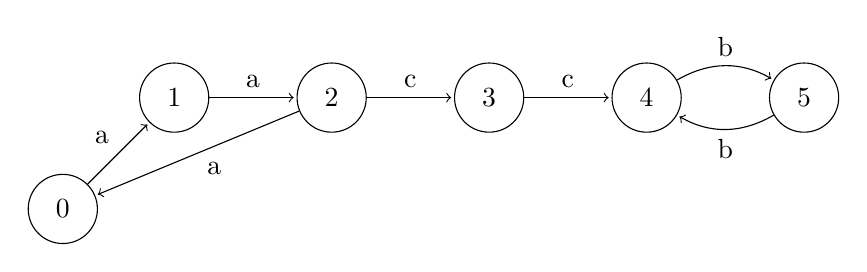
\begin{tikzpicture}[shorten >=1pt,node distance=2cm,on grid,auto] 
   \node[state] (q_0)   {$0$}; 
   \node[state] (q_1) [above right=of q_0] {$1$}; 
   \node[state] (q_2) [right=of q_1] {$2$}; 
   \node[state] (q_3) [right=of q_2] {$3$};
   \node[state] (q_4) [right=of q_3] {$4$};
   \node[state] (q_5) [right=of q_4] {$5$};
    \path[->] 
    (q_0) edge  node {a} (q_1)          
    (q_1) edge  node {a} (q_2)
    (q_2) edge  node {a} (q_0)
    (q_2) edge  node {c} (q_3)
    (q_3) edge  node {c} (q_4)
    (q_4) edge[bend left, above]  node {b} (q_5)
    (q_5) edge[bend left, below]  node {b} (q_4);
\end{tikzpicture}
}
\label{input}
\caption{The input graph}

\end{figure}

\begin{enumerate}
\item Let $\Sigma_{()} =\{ t_( , t_)  | t \in \Sigma \}$.
\item Let $N_{()} = \{ N_( , N_) | N \in N  \}$.
\item Let $M_{\mathcal{G}} = (V_{\mathcal{G}}, E_{\mathcal{G}}, L_{\mathcal{G}})$ is a directed 
labeled graph, where $L_{\mathcal{G}} \subseteq (\Sigma_{()} \cup N_{()})$.
This graph is created the same manner as described in~\cite{OptimalDLR} but we do not require the grammar be in CNF.
Let $x \in V_{\mathcal{G}}$ and $y \in V_{\mathcal{G}}$ is ``start'' and ``final'' vertices respectively. 
This graph may be treated as a finite automaton, so it can be minimized and we can compute an $\varepsilon$-closure if the input grammar contains $\varepsilon$ productions.
The graph $M_{\mathcal{G}}$ for our example is presented in fig.~\ref{mod}.

\begin{figure}
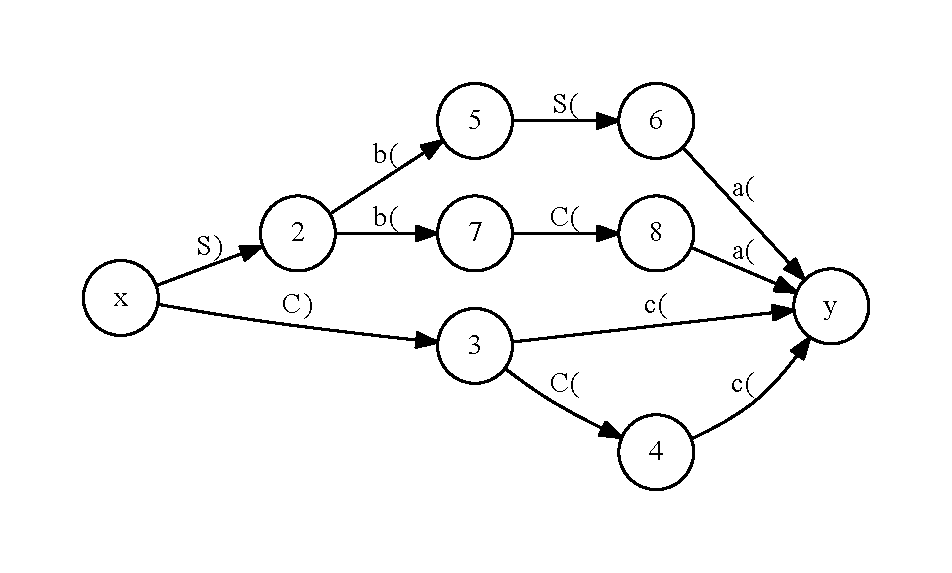
\includegraphics[width=.5\textwidth]{dot/grammar_1.pdf}

\caption{The $M_{\mathcal{G}}$ graph}
\label{mod}

\end{figure}


The minimized graph is presented in fig.~\ref{minimized}.
\begin{figure}
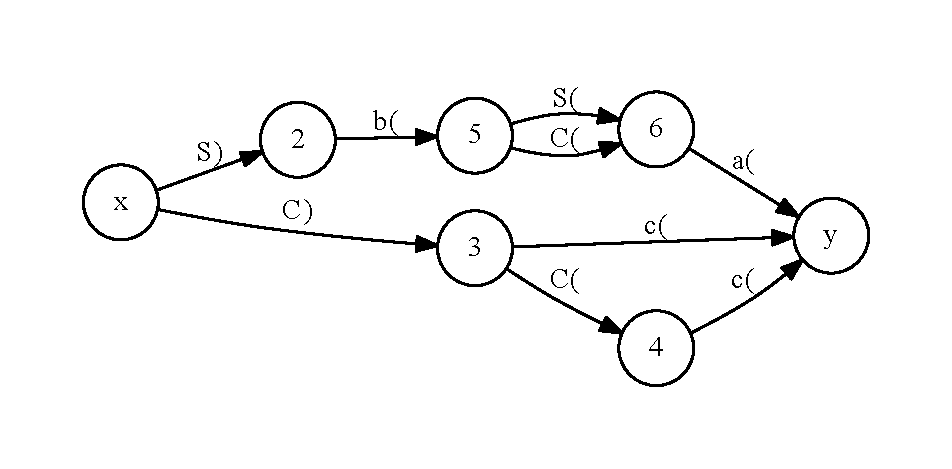
\includegraphics[width=.5\textwidth]{dot/grammar_min.pdf}


\caption{The minimized $M_{\mathcal{G}}$}
\label{minimized}

\end{figure}


\item For each $v \in V$ create $M_{\mathcal{G}}^v$: unique instance of $M_{\mathcal{G}}$.
\item New graph $G^{'}$ is a graph $G$ where each label $t$ is replaced with $t_{)}^i$ and some additional edges are created:
\begin{itemize}
\item Add an edge $(v', S_(, v)$ for each $v \in V$. 
\item And the respective $M_{\mathcal{G}}^v$ for each $v \in V$:
  \begin{itemize}
    \item reattach all edges outgoing from $x^v$ (``start'' vertex of $M_{\mathcal{G}}^v$) to $v$;
    \item reattach all edges incoming to $y^v$ (``final'' vertex of $M_{\mathcal{G}}^v$) to $v$.    
  \end{itemize}
  New input graph is ready. It is presented in fig.~\ref{newInput}.

\begin{figure*}  
  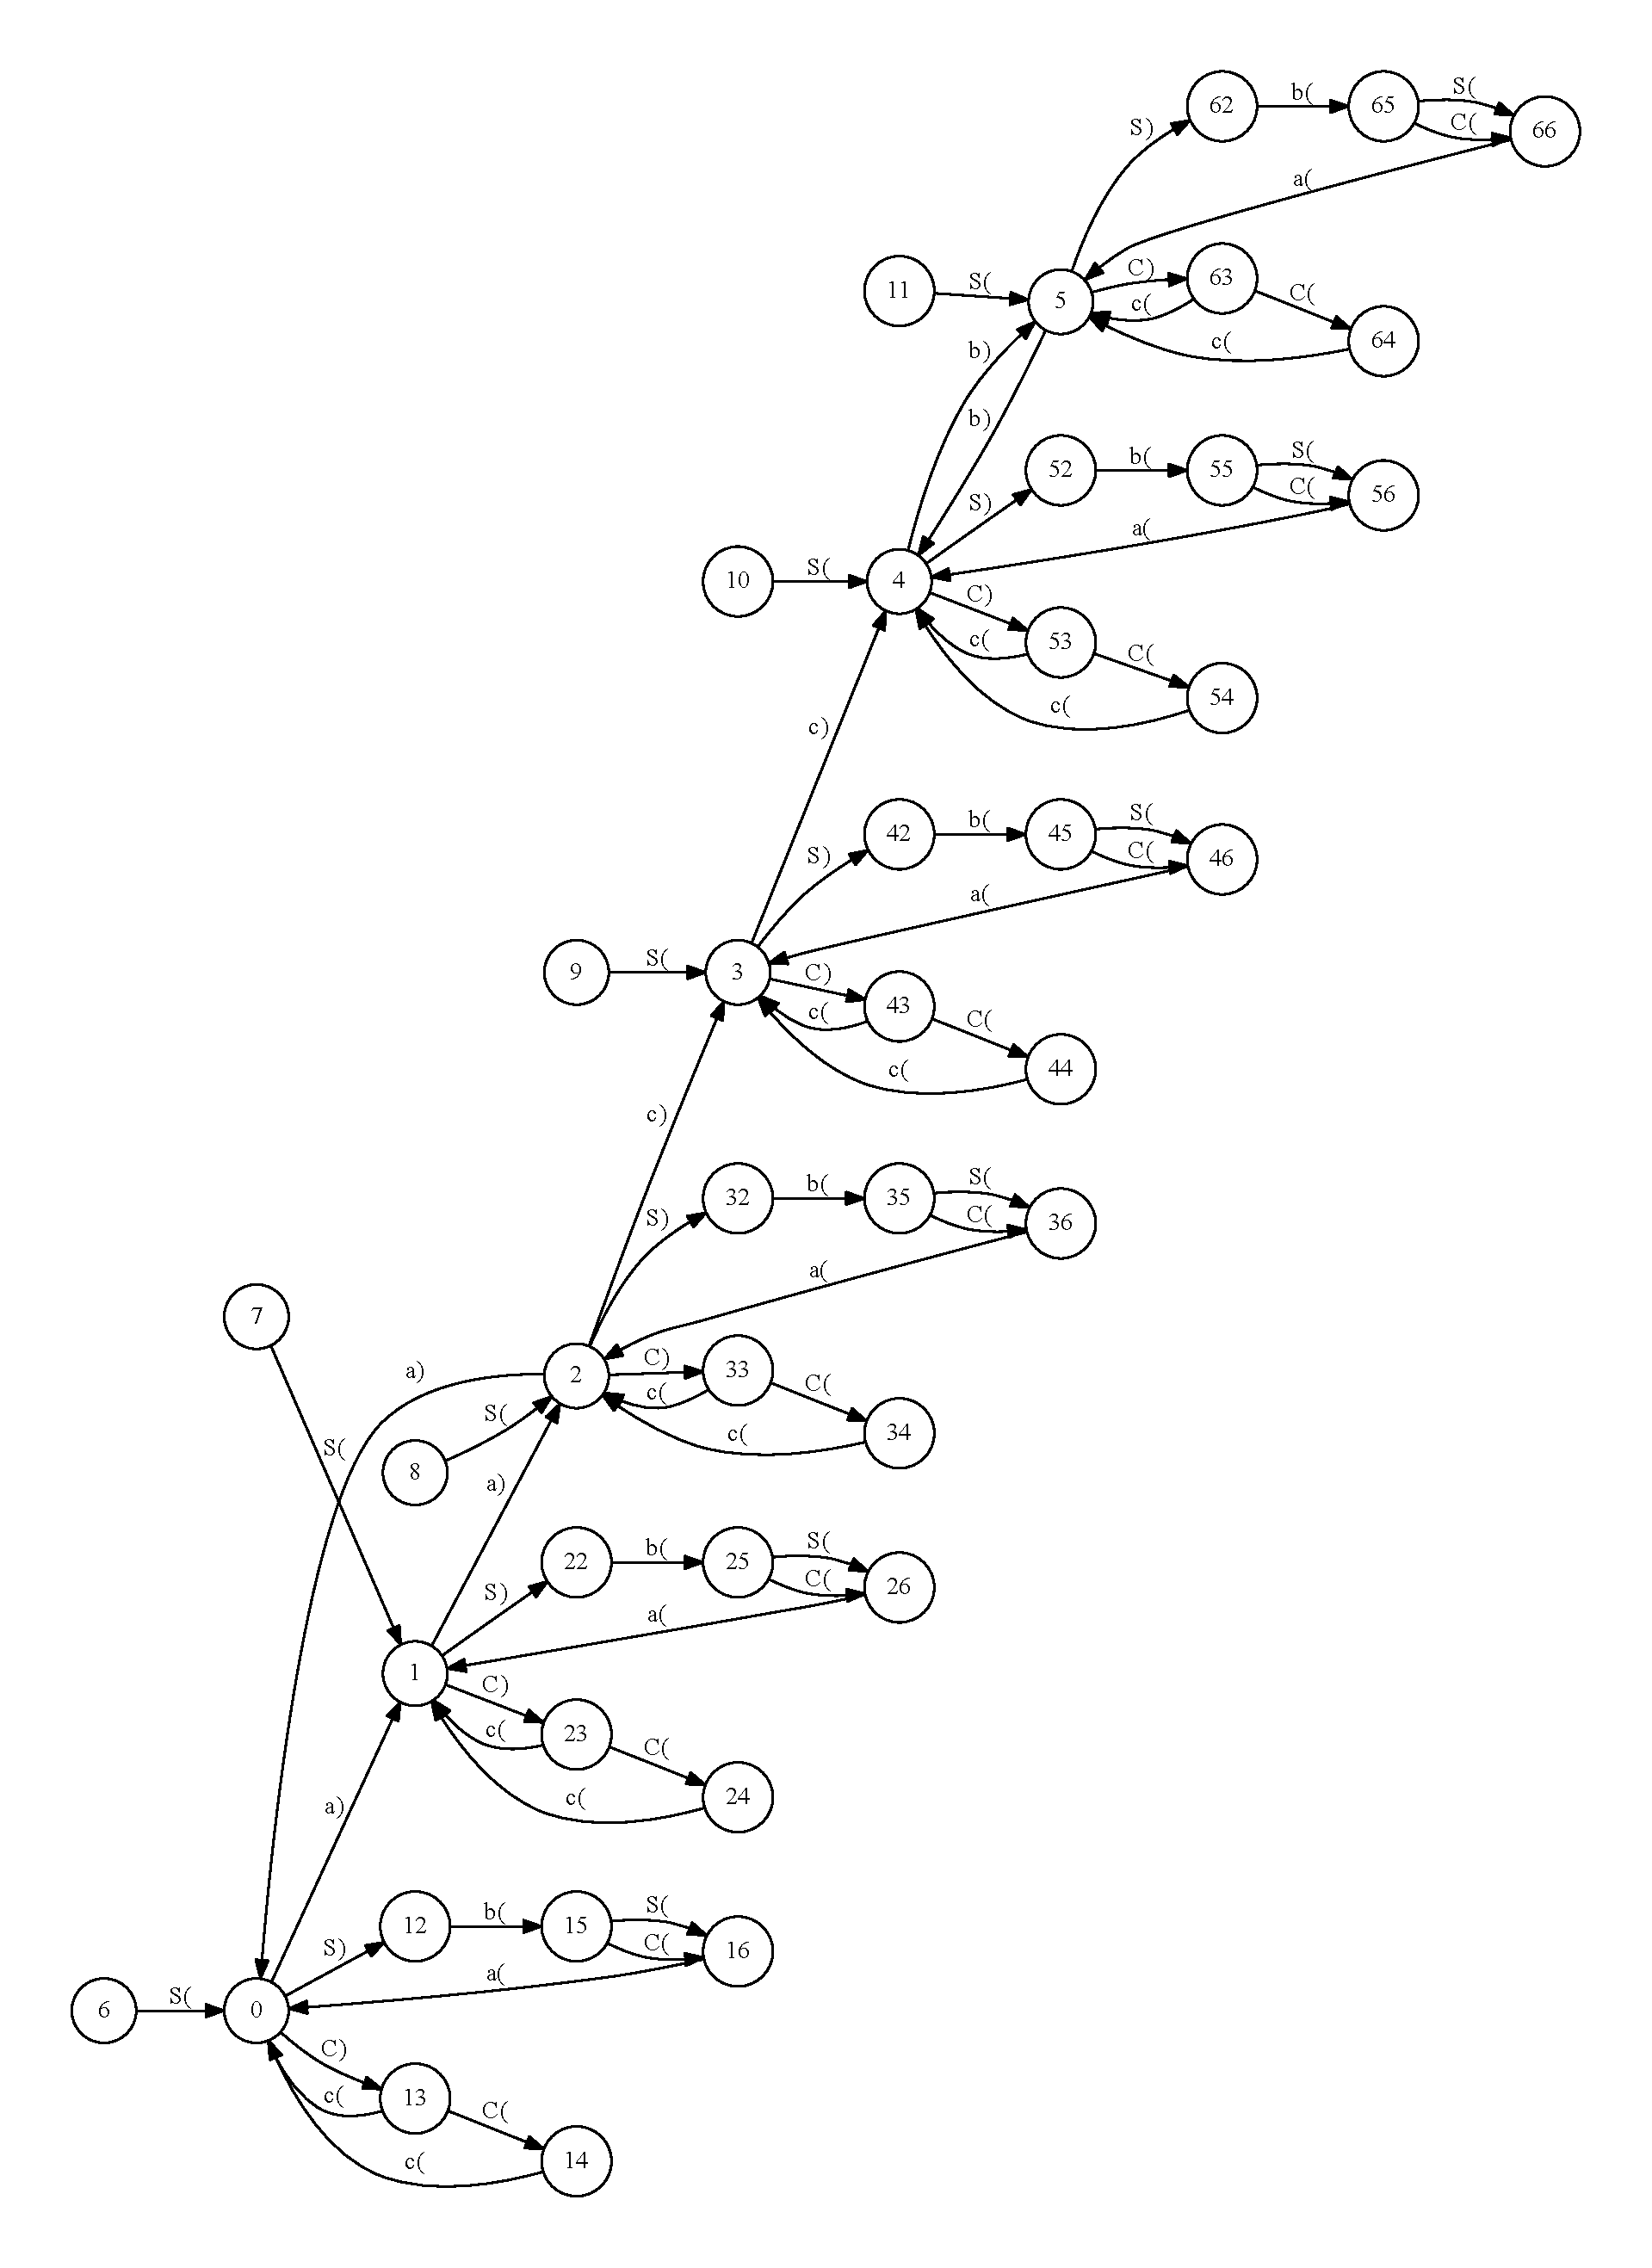
\includegraphics[width=.9\textwidth]{dot/input_new_min.pdf}
 
  \caption{New input graph}
  \label{newInput}

\end{figure*}

\end{itemize}

\item New grammar $\mathcal{G'}=(\Sigma^{'}, N', P', S')$ where $\Sigma^{'} = \Sigma_{()} \cup N_{()}$, $N' = \{ S' \}$, $P' = \{ S' \rightarrow b_( \ S' \ b_); S' \rightarrow b_( \ b_) \ | \ b_(, b_{)} \in \Sigma^{'} \} \cup \{ S' \rightarrow S' \ S' \}$ is a set of productions, $S' \in N'$ is a start nonterminal.
\end{enumerate}

Now, if $\text{CFPQ}(\mathcal{G'}, G')$ contains a pair $(u'_0, v')$ such that $e=(u'_0, S_( , u'_1) \in E'$ is an extension edge (step 5, first subitem), then  $(u'_1, v') \in \text{CFPQ}(\mathcal{G}, G)$.
In our example, we can find the following path: $7 \xrightarrow{S_(} 1 \xrightarrow{S_)} 22 \xrightarrow{b_(} 25 \xrightarrow{C_(} 26 \xrightarrow{a_(} 1   
\xrightarrow{a_)} 2 \xrightarrow{C_)} 33 \xrightarrow{C_(} 34 \xrightarrow{c_(} 2  \xrightarrow{c_)} 3 \xrightarrow{C_)} 43 \xrightarrow{c_(} 3 \xrightarrow{c_)} 4 \xrightarrow{b_)} 5$. 
Edge $7 \xrightarrow{S_(} 1$ is the extension, so (1,5) should be in $\text{CFPQ}(\mathcal{G}, G)$ and it is true.



%\section{two brs}

Let the input grammar is 
\begin{align*}
S & \rightarrow a \ S \ b \ 
\\
S & \rightarrow c \ S \ d \
\\
S & \rightarrow a \ b
\\
S & \rightarrow c \ d
\end{align*}

The input grammar in CNF is 
\begin{align*}
S   & \rightarrow A \ S_1
\\
S_1 & \rightarrow S \ B
\\
S   & \rightarrow C \ S_2
\\
S_2 & \rightarrow S \ D
\\
S   & \rightarrow C \ D
\\
S   & \rightarrow A \ B
\\
C   & \rightarrow c
\\
D   & \rightarrow d
\\
A   & \rightarrow a
\\
B   & \rightarrow b
\end{align*}


Let the input graph is:
\\
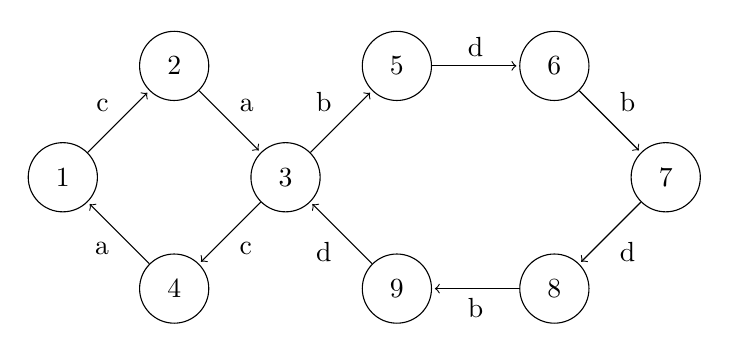
\begin{tikzpicture}[shorten >=1pt,node distance=2cm,on grid,auto] 
   \node[state] (q_1)   {$1$}; 
   \node[state] (q_2) [above right=of q_1] {$2$}; 
   \node[state] (q_3) [below right=of q_2] {$3$}; 
   \node[state] (q_4) [below right=of q_1] {$4$};
   \node[state] (q_5) [above right=of q_3]  {$5$}; 
   \node[state] (q_6) [right=of q_5] {$6$}; 
   \node[state] (q_7) [below right=of q_6] {$7$}; 
   \node[state] (q_9) [below right=of q_3] {$9$};
   \node[state] (q_8) [right=of q_9] {$8$};

    \path[->] 
    (q_1) edge  node {c} (q_2)          
    (q_2) edge  node {a} (q_3)
    (q_3) edge  node {c} (q_4)
    (q_4) edge  node {a} (q_1)

    (q_3) edge  node {b} (q_5)          
    (q_5) edge  node {d} (q_6)
    (q_6) edge  node {b} (q_7)
    (q_7) edge  node {d} (q_8)
    (q_8) edge  node {b} (q_9)
    (q_9) edge  node {d} (q_3)
    
    ;
\end{tikzpicture}




%\bibliographystyle{abbrv}
\bibliographystyle{ACM-Reference-Format}
\bibliography{SAT_to_CFPQ}



\end{document}